% !TEX root = ../../../main.tex
% 来源：高中物理甲种本·第三册（电磁·光学·近代物理）
% 章节：交流电 / 表征交流电的物理量
% 原始文件：3.tex，行 279-291
% 类型：tikz
% ---
    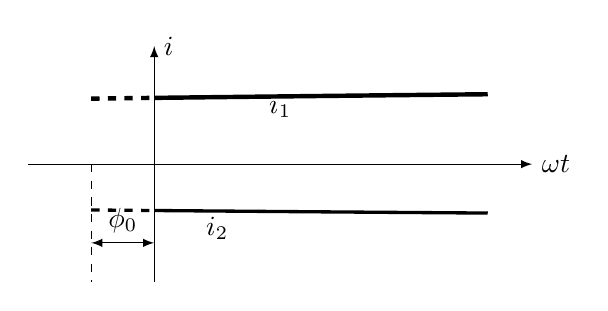
\begin{tikzpicture}[>=latex, xscale=.8]
        \draw [->](-2,0)--(6,0)node[right]{$\omega t$};
        \draw [->](0,-1.5)--(0,1.5)node[right]{$i$};
        \draw [ultra thick] plot[domain=0:5.3, samples=1000, variable=\x] (\x, {sin(\x+1 r)}) ;
        \draw [ultra thick, dashed] plot[domain=-1:0, samples=100, variable=\x] (\x, {sin(\x+1 r)});
        \node at (2,1) [below]{$i_1$};
        \draw [very thick] plot[domain=0:5.3, samples=1000, variable=\x] (\x, {-.7*sin(\x+1 r)}) ;
        \draw [very thick, dashed] plot[domain=-1:0, samples=100, variable=\x] (\x, {-.7*sin(\x+1 r)});
        \node at (1,-.55)[below]{$i_2$};
        \draw [dashed] (-1,0)--(-1,-1.5);
        \draw [<->] (0,-1)--node[above]{$\phi_0$}(-1, -1);

\end{tikzpicture}
